\documentclass[a4paper,10pt]{scrartcl}

% Deutsche Umlaute (Mac)
\usepackage[applemac]{inputenc}

% Deutsche Umlaute (Windows)
%\usepackage[ansinew]{inputenc}

% Einbinden von Bildern
\usepackage{graphicx}

% SeitenflŠche etwas mehr ausnutzen
\usepackage{geometry}
\geometry{a4paper,left=30mm,right=30mm, top=1cm, bottom=3cm}

% Kein EinrŸcken bei zweispaltigen Bildunterschriften
\usepackage[normal]{caption}

% == Lottes Änderungen ===
\usepackage{todonotes}
\usepackage{hyperref}
\usepackage{wrapfig}

% großer erster Buchstabe
\usepackage{lettrine}
\usepackage{graphicx}
\usepackage{caption}
\usepackage{subcaption}

% Glossary benutzen
\usepackage{glossaries}
\loadglsentries[main]{glossary}
\makeglossaries

% zeilenumbrüche in tabellen
\newcommand{\specialcell}[2][c]{%
  \begin{tabular}[#1]{@{}c@{}}#2\end{tabular}}

\begin{document}

% Titel
\title{Hybrid routing for the Internet of Things}
\subtitle{challenges and opportunities}
\author{Lotte Steenbrink}
\date{Wintersemester 2014/15}
\maketitle

\begin{abstract}
%I am an abstract. Write me!
With the \gls{IoT}, new use cases and requirements for mobile mesh networks have begun to blossom. In order to meet these requirements, routing protocols are needed to manage connectivity and prepare the transport of packets. Traditionally, proactive protocols have been used for environments with more traffic and high constraints in terms of latency, while reactive protocols have been used for sparse, high-mobility networks. IoT networks may exhibit all of the aforementioned characteristics at the same time, or change from one set to another depending on their environment. This is why neither pure proactive or reactive routing may be able to satisfy the IoT's demands: Protocols need to be able to adopt to a rapidly changing environment, and do so autonomously and efficiently.
Because traditional approaches to routing may not be feasible for this task, \emph{hybrid roting protocols} have begun to resurface. This paper will introduce existing approaches to hybrid routing and aims to provide suggestions on how to evolve them to make them a better fit for the IoT.

\end{abstract}

\section{Introduction}
\label{sec:Intro}
%==============================================================================

\subsection{What is the Internet of Things?}
\label{subsec:IoT}
%==============================================================================
The \gls{IoT} envisions autonomous communication between computers installed in everyday objects such as furniture, toys, clothing, or tools with the goal of making them smarter and improving their user experience. Some IoT devices are very constrained, with no constant power supply. Therefor, they need to be resourceful in terms of computation, storage, RAM and energy usage. Other devices may not exhibit one or any of these characteristics. For example, a sensor built into a lamp can tap into the available power supply and is therefor not restricted by battery life concerns. A computer controlling a smart home may have more computation resources than the IoT nodes it manages, and so on. In other words, IoT networks are comprised of hardware which are homogeneous in terms of abilities and requirements, but most nodes are constrained in some way.\\

To communicate amongst each other, IoT nodes form spontaneous, wireless mesh networks.
The vision of the Internet of Things is rapidly becoming reality, and with its rise, environments which cannot be optimally served by either reactive or proactive routing protocols alone are created. Thus, the demand for a new kind of routing protocol is created, too.\\
One example for this may be the lighting system in a smart home: Each lamp needs to maintain a stable connection to the control center of the house. This means that a substantial amount of control traffic is directed at the sink node that is the central control. Because of its direction, this traffic forms a tree-like topology. In addition to this, lamps may want to communicate spontaneously between each other, for example to create optimal lighting in the study when homeowners sit down at their desk.

\subsection{What is Hybrid Routing?}
\label{subsec:hybrid}
%==============================================================================
Hybrid Routing protocols combine two central routing paradigms in one protocol: Reactive and proactive routing. While reactive protocols stay idle until a route is needed and then \emph{react} to this demand, proactive protocols constantly monitor their network for peers and link qualities, (re-)calculating routes as they gather new data. The former class of protocols perform well in sparse, very mobile networks and save energy by generating less control overhead. The latter are best suited for networks with high demands in terms of throughput, reliability and latency.\\
Hybrid routing protocols aim to adjust their routing strategy from proactive to reactive and, conversely, from reactive to proactive, depending on the circumstances: Routes or areas that are deemed important or see a lot of traffic require proactive attention, while sparsely, less important or very mobile areas or routes are best served reactively.\\
In the example of section \ref{subsec:IoT}, all lamps would maintain a proactive route towards the control center, while inter-lamp communication may be set up reactively.\\

The rest of this paper is organized as follows. \todo{TODO! double-check!}
In the next section, requirements for a hybrid routing protocol will be listed, followed by an introduction to key aspects of hybrid routing protocols. Section \ref{sec:existing_protocols} will then go into the specifics of existing protocols, and how they exhibit these characteristics. Following up, section \ref{sec:suitability} will discuss which of these aspects and protocols are the most promising for the IoT, and section \ref{sec:experiments} will explain how this has been and will be verified through experiments. Finally, sections \ref{sec:conclusion} and \ref{sec:outlook} will provide a conclusion and an outlook towards future work.

\section{the history of hybrid protocol research}
\label{sec:related_work}
%==============================================================================
Most research on hybrid routing protocols stems from an era where wireless mesh routing was at its very beginning. This meant that the building blocks for hybrid routing, namely proactive and reactive routing protocols, were under construction themselves. While proactive and reactive protocols were developed and examined, research in hybrid routing stalled until a more thorough understanding of proactive and reactive has been reached.\\
This has since been achieved: The \gls{IETF} has standardized \gls{OLSR}\cite{RFC-3626}, OLSRv2\cite{RFC-7181} and \gls{AODV}\cite{RFC-3561}, AODVv2\cite{draft-ietf-manet-aodvv2-06} is on its way to become a standard, and \gls{LOADng}\cite{draft-yi-loadngct-02} will be deployed in the large-scale smart grid network of France \cite{X800}. The body of experience with both reactive and proactive protocols has grown and created the building blocks needed to pick up hybrid routing protocol research again.\\

But while this milestone has been reached, the amount of protocols of any kind specifically targeted at IoT-like environments is very small. By the time of this writing, the \gls{RPL}\cite{RFC-6550} is the only dedicated IoT protocol available, and it cannot cover the entire diverse set of requirements that are found under the umbrella term of ``Internet of Things''. Thus, it is necessary to evaluate protocols designed for environments that share some characteristics with the Internet of Things and may be customized to be a good fit. Suitable environments are as follows:
\begin{description}
\item[\glspl{DTN}] are designed to cope with network partitioning, which my be caused by movement or lossy links.
\item[\glspl{MANET}] share the characteristic mobility challenges and ad-hoc nature of their infrastructure with the IoT.
\item[\glspl{LLN}] match IoT requirements the closest: nodes are expected to be constrained in terms of battery and computation resources, and links are expected to be lossy. One might say that The IoT consists of many LLNs, attached to the big Internet through border routers.
\item[\glspl{VANET}] have seen a lot of research concerning hybrid protocols. Unfortunately, their characteristics differ too drastically from the IoT: node mobility in VANETs is extremely high, with somewhat ordered movement patterns as cars usually only move on streets, which are known beforehand. %And because it has access to the energy system of a car, battery life is not as critical.
\end{description}

The goal of this paper is thus to explore how hybrid routing can be advanced with the \gls{IoT} in mind, building on the foundation which research on \gls{MANET} routing of the past 15 years has built. It aims to provide a critical overview over existing work and highlight challenges which might arise in hybrid protocol design for the IoT.\\

\section{Requirements for hybrid IoT routing protocols}
\label{subsec:requirements}
%...............................................................................
Ramasubramanian et al. \cite{SHARP} list three core properties a hybrid routing protocol needs to have. Although originally written with mobile ad-hoc networks in mind, these principles can be adapted to the IoT.
\begin{description}
\item[Adaptivity] Because IoT use cases are as numerous as its environments are subject to changes, the protocol should be able to adapt to a wide variety of circumstances. It should adjust its behavior to changes in mobility, traffic patterns, link quality, and other qualities.
\item[Flexibility] The protocol should be able to satisfy the requirements of different applications in terms of reliability, latency or throughput.
\item[Efficiency and robustness] The protocol should strive to be efficient in terms of energy consumption, traffic and computational overhead, all the while maintaining the ability to reliably find routes through the network. It must perform equally well or better than purely reactive or proactive protocols in the same situation.
\end{description}

\section{Existing Protocols}
\label{sec:existing_protocols}
%-------------------------------------------------------------------------------
The following section will provide a short introduction to all existing hybrid routing protocols and its characteristic mechanisms for \glspl{MANET}, \glspl{LLN} and \glspl{DTN}. A tabular overview can be found in table \ref{fig:overview}.

\begin{table*}[t]
    \begin{tabular}{p{0.5\textwidth}|l|l|l}
        Name & Scope & Architecture & Published \\
        \hline
        Node-Centric Hybrid Routing \cite{Roy_nodecentric} & Path & Compositional & 2002 \\ % proactive fixed
        SHARP\cite{SHARP} & Area and path & Compositional & 2003 \\ %TODO: only for reactive!
        P2P extension\cite{RFC-6997} of RPL\cite{RFC-6550} & Path & Monolithic & 2013\\
        ZRP \cite{ZRP-Draft} and extensions \cite{TZRP} \cite{IZR} \cite{WARP} & Area & Monolithic & 2002/2004\\
%        \gls{WARP}\cite{WARP} & Area and Path & Protocol & 2002\\ % TODO: evtl doch mit reinnehmen und auseinandernehmen?
        ZHLS\cite{ZHLS} & Area & Monolithic & 1999\\
        HYMAD\cite{HYMAD} & Area & Compositional & 2010\\ % Only DTN protocol is variable!
    \end{tabular}
    \caption{Overview over existing hybrid protocols. An explanation of the terminology used can be found in section \ref{sec:key_aspects}}
    \label{fig:overview}
\end{table*}

%\newpage % TODO maybe remove me

\subsection{\gls{ZRP}}
\label{subsec:zrp}
%...............................................................................

\begin{wrapfigure}{r}{0.5\textwidth}
  \begin{center}
    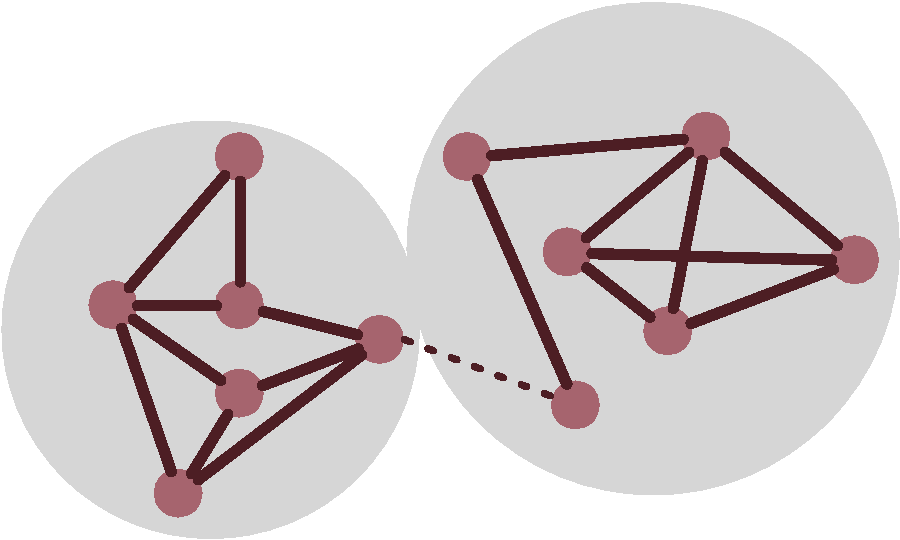
\includegraphics[width=0.48\textwidth]{../images/ZRP}
  \end{center}
  \caption{Sketch of area-centered routing, as practiced by ZRP, ZHLS and HYMAD}
  \label{fig:zrp_area_centered}
\end{wrapfigure}

The Zone Routing Protocol was originally developed for \glspl{MANET} and is one of the most-referenced and -extended hybrid routing protocols to date. It was originally described in an Internet-draft which expired on January 2003\cite{ZRP-Draft}.
It clusters nodes into so-called \emph{Routing Zones}, which adapt their diameter to the network's degree of mobility and traffic density. Routes inside these routing zones are discovered and maintained in a proactive fashion. In addition to the topology inside their zone, nodes are also aware of topology which all routing zones form.
To find routes to nodes in foreign routing zones, the reactive protocol makes use of a technique similar so some multicast routing approaches. The so-called \gls{BRP}\cite{draft-ietf-manet-zone-brp} protocol constructs a \emph{bordercasting} tree between all routing zones, and forwards the packet along the tree to one \emph{bordercasting node} per routing zone. Each bordercasting node will know if the target of the route discovery is in their routing zone, since the zones are maintained with a proactive protocol. If this is the case, it reports this to the source node, and the data exchange begins. If it is not the case, it forwards the packet. This way, traffic overhead is avoided. An illustration of this clustering can be found in fig. \ref{fig:zrp_area_centered}\\
The draft describes ZRP as a routing \emph{framework}. It introduces its own proactive and reactive protocol, namely the \gls{IARP}\cite{draft-ietf-manet-zone-iarp} for proactive routing inside routing zones, and the \gls{IERP}\cite{draft-ietf-manet-zone-ierp} to discover routes between zones reactively. Because of the modular nature of ZRP, alternate protocols such as OLSR for proactive or AODV for reactive may be used instead of the predefined options (i.e. IERP and IARP).\\
There are two extensions of ZRP: the \gls{TZRP}\cite{TZRP}, the \gls{WARP}\cite{WARP} and the \gls{IZR}\cite{IZR}.

\subsection{\gls{ZHLS}}
\label{subsec:zhls}
%...............................................................................
ZHLS is a hierarchical, GPS-based roting protocol.
ZHLS clusters all nodes into non-overlapping routing zones based on their location. These clusters form a hierarchy, with the nodes at its very bottom.
On startup, each node determines their location and joins the zone which spans across the area they're in. Route discovery within the zones is done in a proactive fashion. Whenever a packet needs to travel outside the cluster, it is routed along the zone hierarchy. Because there are no cluster heads, a lot of flooding happens. \todo{disentangle the general WTFness of this protocols's operation}
This protocol design bears the often erroneous assumption that physical proximity guarantees near-optimal connectivity, which has been debunked by \cite{mistaken-axioms}. \todo{go into troubles of georouting?}
\cite{ZHLS-GF} reintroduces the 

\subsection{Node-Centric Hybrid Routing}
\label{subsec:nchr}
%...............................................................................
NCHR\cite{Roy_nodecentric} serves networks which contain some nodes, called \emph{netmarks}, that offer services to their peers, such as being a DNS server or an Internet Access Point. All nodes in the network maintain proactive routes towards the netmarks, while other connections are established reactively. The draft uses SOAR\cite{SOAR} for this, but maintains that AODV\cite{RFC-3561} or DSR\cite{DSR} may be used just as easily.
Hamma et al.\todo{elaborate} propose to reintroduce gateway flooding to ZHLS.

\subsection{\gls{HYMAD}}
\label{subsec:hymad}
%...............................................................................
Just like ZRP, ZHLS, and Node-centric Hybrid routing, nodes participating in HYMAD \cite{HYMAD} form proactively maintained zones. These zones are maintained by an unspecified distance-vector routing algorithm.
The difference to all previously named protocols is that HYMAD borrows its approach to inter-zone roting not from traditional \gls{MANET} schemes, but from Delay-Tolerant Networks (DTN), where nodes store data until they move and meet other nodes with which they can communicate (this is called \emph{store-and-forward}).\\
While amongst the more recent research, there are no peer-reviewed publications about HYMAD.

%todo wie genau bin ich darauf gekommen dass das ein framework ist?

%\newpage % TODO maybe remove me

\subsection{\gls{SHARP}}
\label{subsec:sharp}
%...............................................................................
\begin{wrapfigure}{r}{0.5\textwidth}
  \begin{center}
    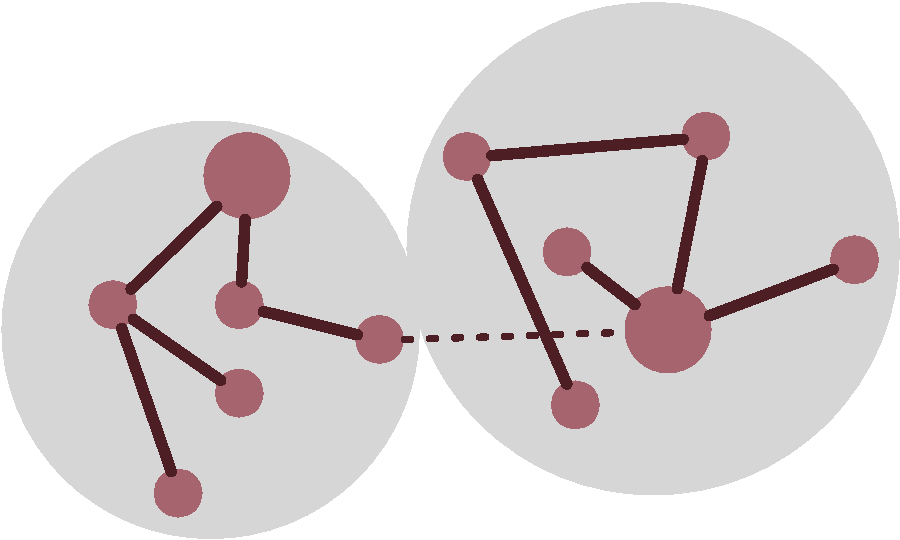
\includegraphics[width=0.48\textwidth]{../images/SHARP}
  \end{center}
  \label{fig:area_centered}
  \caption{Sketch of the SHARP topology}
\end{wrapfigure}

This protocol claims to offer each application the possibility to specify their needs in terms of latency and loss rate in the form of a metric, which is then used to guide the trade-off between proactive protocol overhead and reactive loss of reliability and latency.
SHARP combines both area-centered and path-centered paradigms in what could be called a path-centered-in-area-centered approach. Routing zones are established around \emph{hot destinations}, i.e. nodes at which a majority of the traffic is directed. Gateways, nodes that offer a service, or sink nodes which collect sensor data in a Wireless Sensor Network may qualify as such a hot destination. Inside these routing zones, a \gls{DODAG} is formed with the hot destination as root, and proactive routes are kept \emph{only towards the hot destination node}. SHARP claims that this help meet the application requirements stated above, but it comes at the cost of enhanced traffic overhead and uneven battery draining, because nodes closer to the hot destination will forward more traffic than the ones on the outskirts.\\
If the desired destination is outside of the routing zone, a reactive route discovery is initiated. This is similar to ZRP's approach.\\
SHARP's routing strategy relies heavily on the assumption that only special nodes are the target of traffic, and is likely to fail in environments where all nodes are equal.\\
SHARP defines its own proactive protocol, the SHARP Proactive Routing protocol (SPR), which is based on DSDV\cite{DSDV} and TORA\cite{TORA}. Neither of these protocols are relevant in MANET routing as of today.
For reactive routing, AODV is used, but may be exchanged for any other reactive protocol.\\
\cite{SHARP} does not offer a solution as to how hot destinations may be identified by the participating nodes.

\subsection{P2P-RPL}
\label{subsec:p2prpl}
%...............................................................................
\begin{wrapfigure}{r}{0.5\textwidth}
  \begin{center}
    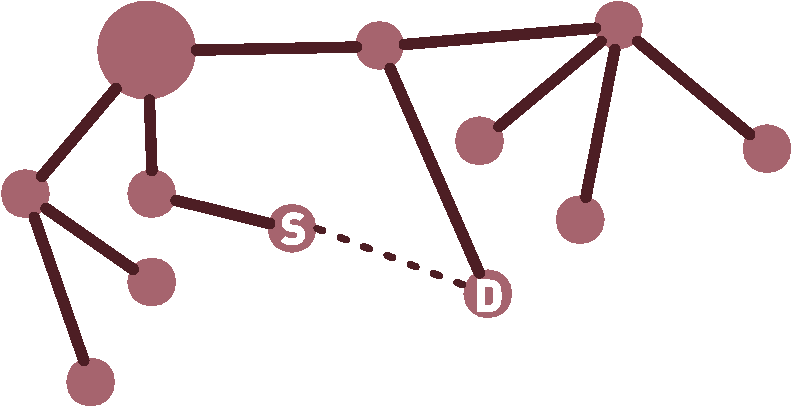
\includegraphics[width=0.48\textwidth]{../images/p2pRPL}
  \end{center}
  \label{fig:p2p}
  \caption{Sketch of the P2P-RPL topology}
\end{wrapfigure}

The P2P-RPL protocol is an extension of the IPv6 Routing Protocol for Low-Power and Lossy Networks (RPL)\cite{RFC-6550}. RPL itself was designed for IoT-like circumstances, but focus primarily on networks which feature a \emph{sink node} towards which all traffic is directed. RPL constructs a \gls{DODAG} whose root is the sink node. All traffic is then routed towards the sink node. Parent nodes in the DODAG do not necessarily know about their children, so communication towards any other than the sink node is not possible in all configurations of the RPL protocol. In case it is possible, packets from one leaf node to another will always have to travel to the root node first to be sent back, even if they are in close proximity. In networks with a substantial amount of peer to peer traffic, this leads to battery draining and traffic bottlenecks close to the sink node. This is why \cite{baccelli_p2p_rpl} suggests to extend the protocol with reactive route request messages which are piggybacked onto regular RPL traffic whenever a node S wants to communicate with a neighbor D, which is not the sink node. As soon as it receives this route request, D answers with a route reply. Through the distribution of these messages, a DODAG originating at S is formed, along which the peer to peer traffic can now be routed.

\section{Key aspects of Hybrid Routing Protocols}
\label{sec:key_aspects}
%==============================================================================
All hybrid protocols discussed in section \ref{sec:existing_protocols} share commonalities, some of which fundamentally shape the way a routing protocol sees and serves a network. The goal of this section is to identify these key aspects and discuss them with regard to the requirements of IoT environment.\footnote{Note that the taxonomies presented are not common in previous work, but were created by the author due to a lack of naming in other literature.}

\subsection{Scope}
\label{subsec:scope}
%==============================================================================

\begin{figure}
        \centering
        \begin{subfigure}[b]{0.5\textwidth}
                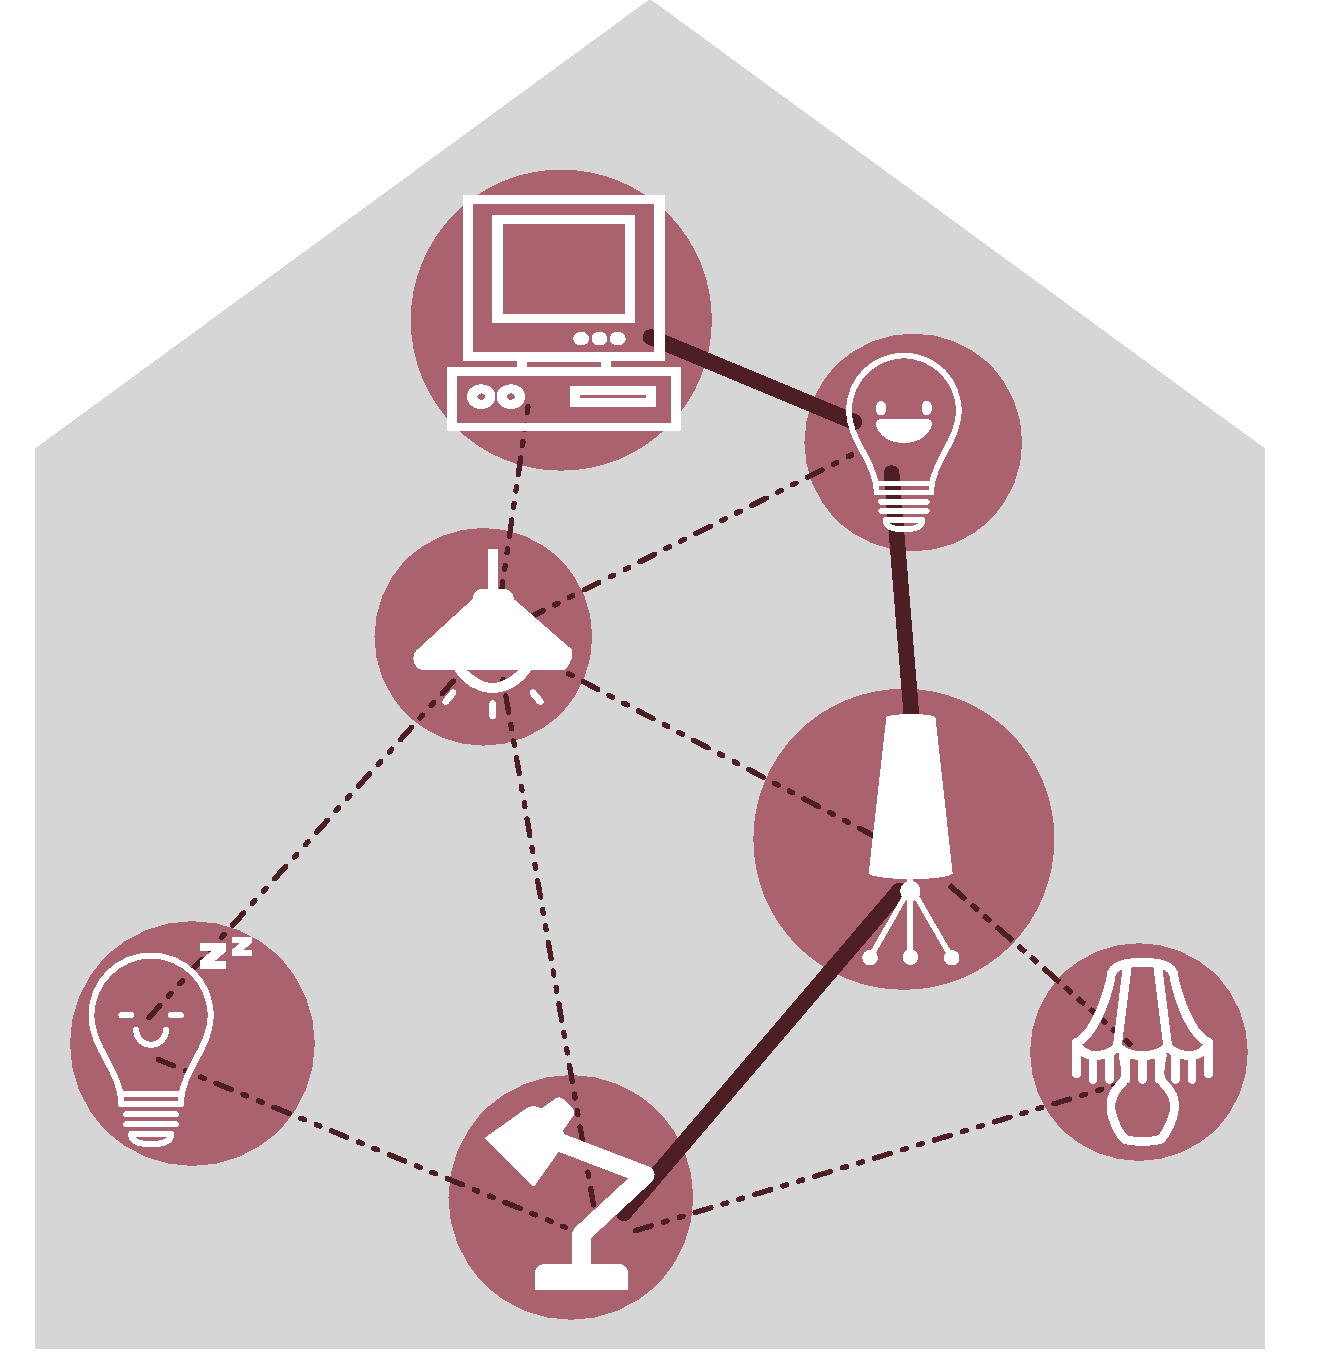
\includegraphics[width=\textwidth]{../images/route_centered_example}
                \caption{Example of a path-centered network: lights and control center in a smart home.}
                \label{fig:rc_img}
        \end{subfigure}%
        ~ %add desired spacing between images, e. g. ~, \quad, \qquad, \hfill etc.
          %(or a blank line to force the subfigure onto a new line)
        \begin{subfigure}[b]{0.5\textwidth}
                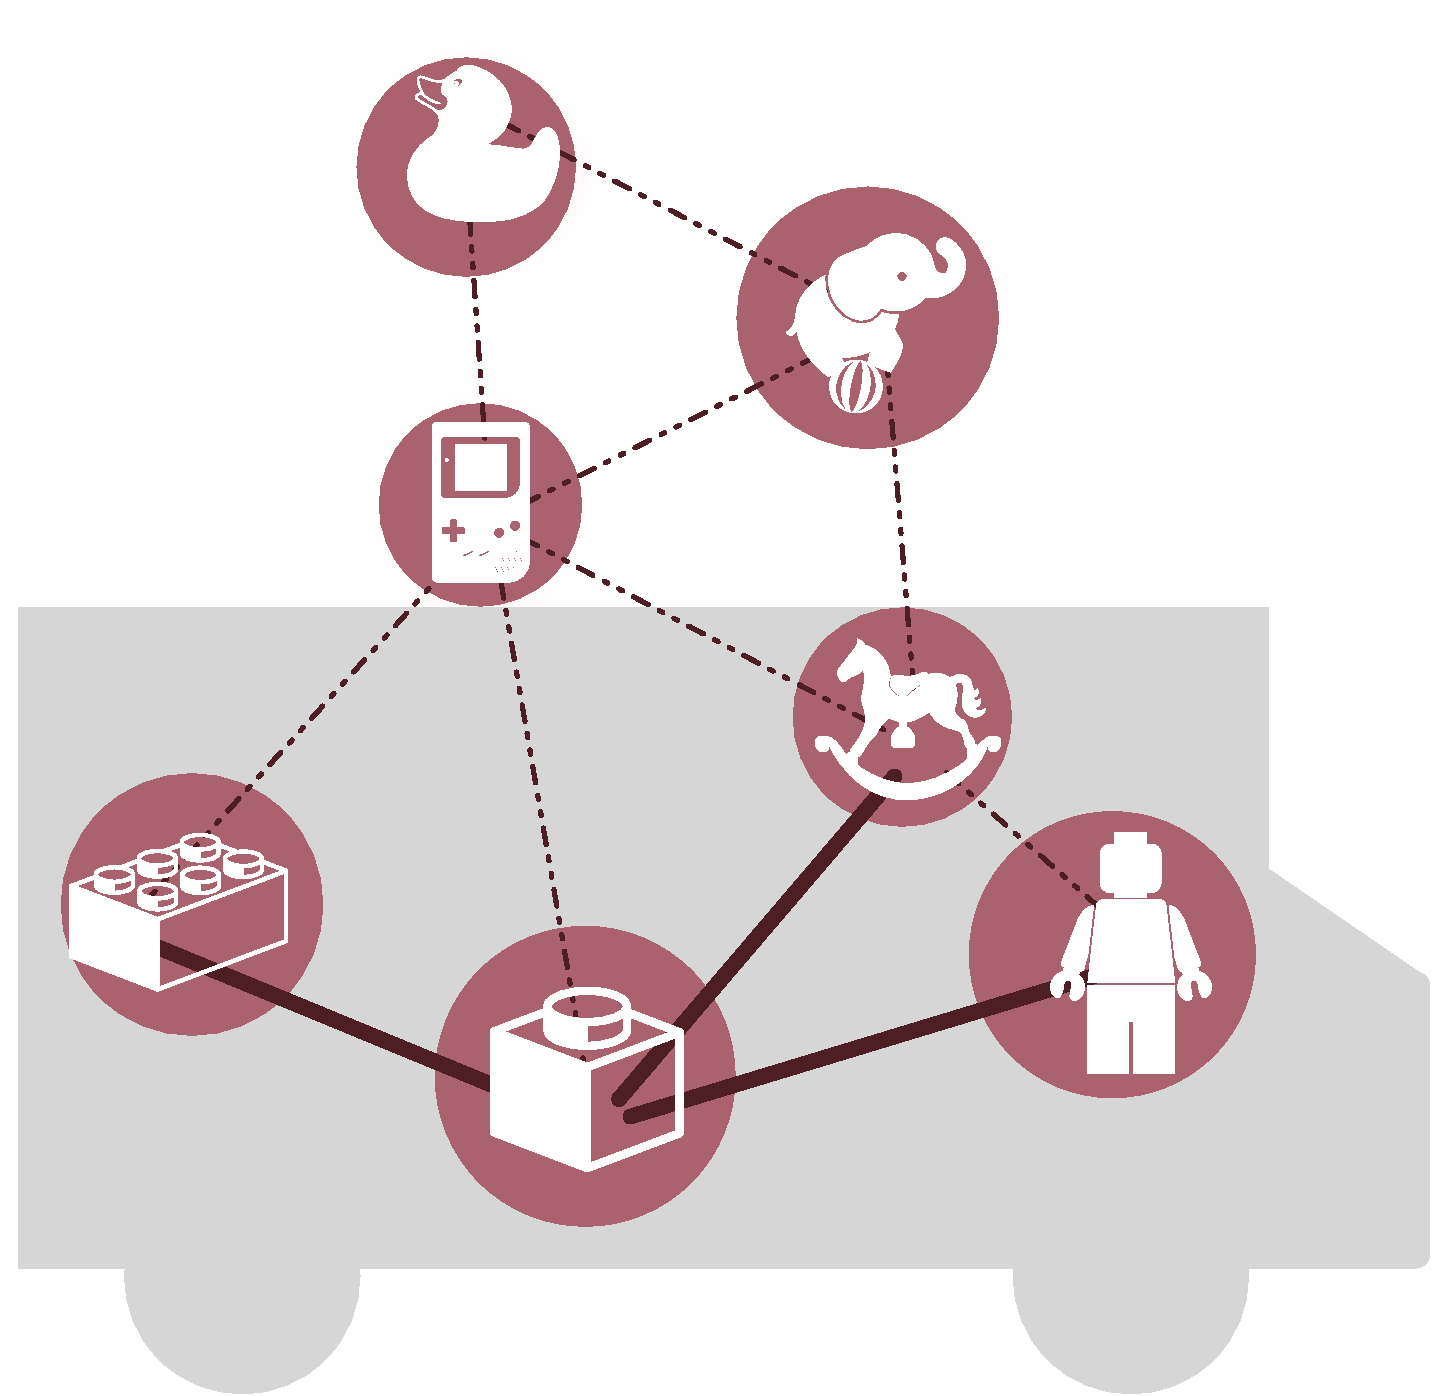
\includegraphics[width=\textwidth]{../images/area_centered_example}
                \caption{Example of an area-centered network: Goods in a delivery truck and warehouse}
                \label{fig:ac_img}
        \end{subfigure}
        \caption{Application Scenarios for hybrid routing protocols}\label{fig:scope}
\end{figure}
\todo{add thenounproject credits}

Hybrid protocols differ in the way they prioritize routes and decide which of them should be maintained proactively or set up reactively. There are two approaches to this, which this paper dubs the \emph{path-centered} and the \emph{area-centered} approach repectively.\\

\begin{description}
\item[path-centered] This approach serves networks in which some nodes, near or far, are more important than others. This is illustrated by fig. \ref{fig:rc_img}, which shows the different lamps of a house and the house's control center. Each lamp needs a stable connection to this control center, be it to switch on/off occasionally to confuse burglars, or exchange status info and configurations. Thus, this connection is maintained proactively, as indicated in the diagram by the thick straight line. Additionally, they may want to communicate with each other upon user interaction. Because this happens spontaneously and sparsely, the connections amongst all lamps are set up reactively, as indicated by the dotted lines.
The most recent publication on hybrid routing, which is also the only publication with a focus on the IoT \cite{RFC-6997}, features a path-centered approach using \gls{RPL}\cite{RFC-6550} as a basis, extending it with its own reactive mechanism.
\\
\item[area-centered] Protocols relying on this approach assume all nodes are equal in principle, but nearby nodes are more important than nodes which are farther away and know their neighborhood best. They cluster the network into so-called ``routing zones''. Nodes that are in the same zone maintain their connections among each other proactively, so routes towards other members of a routing zone are always known beforehand. Routes towards nodes from foreign zones are established reactively. \todo{write about intra-zone routing, border nodes etc}
One example application for this may be a warehouse as illustrated in \ref{fig:ac_img} whose goods (or their packaging) are equipped with IoT hardware. Employees are thus able to tell details about the stock simply by asking their scanner, which communicated with the other IoT devices. In case a truck with new goods arrives, employees can use their scanner to ask for the nearest packaging for information about the entire truckload. Thus, knowledge about their immediate neighbors is vital to these nodes, while none of them has special features which may turn it into a ``more important node''. Many early attempts at Hybrid routing, most popularly \gls{ZRP}, but also more recent research such as HYMAD, feature this approach.
\end{description}

\todo{what about combinations of the two?}

Because the IoT is an umbrella term for many different use cases, none of these approaches is necessarily better than the other. Which approach is suitable depends on traffic patterns (caused by different usage scenarios) and the roles of all nodes involved.%\todo{what about mobility and mobility patterns?}

\subsection{Architecture}
\label{subsec:architecture}
%==============================================================================
Because hybrid protocols incorporate proactive and reactive protocols as building blocks, the relationship between its reactive and proactive components-- how it all goes together-- may be more than just a sequence of instructions. All hybrid protocols presented in section \ref{sec:existing_protocols} can be classified as one of the two following architectural types.
\begin{description}
\item[Monolithic] protocols have a reactive and a proactive component firmly in place. Oftentimes, these components are variations of well-known proactive and reactive protocols, customized to improve the hybrid protocol's overall performance or decrease traffic- or computational overhead. For example, \cite{baccelli_p2p_rpl} piggybacks reactive control traffic onto already existing, proactive RPL messages, thus avoiding unnecessary traffic and saving battery life. %\todo{mehr Beispielprotokolle auflistem}
This bears great potential for optimization, but complicates code re-use and the deployment of updates.\\
\item[Compositional] protocols are organized as a mere \emph{framework} which can be used to combine different proactive or reactive protocols. 
The choice which proactive and reactive protocols are used is not made the protocol designer anymore, but by the person deploying the protocol for a specific environment.\\
Some existing hybrid solutions such as SHARP, Node-Centric Hybrid Routing and HYMAD chose this route, but with a twist: one component, for example the reactive protocol, is fixed, while the proactive protocol can be exchanged at will. This architecture allows for a great deal of flexibility: If a new version of a protocol that is in use surfaces, it can be adopted quickly. The same with alternative protocols which prove to serve some or all use-cases better. Existing implementations of well-known proactive or reactive protocols can be integrated and re-used.
A compositional protocol bears the possibility to be customized for certain deployments, because the most suitable proactive and reactive protocols for the task may be picked and combined seamlessly.
Of course, this comes at the cost of lightweightedness: Approaches which are very flexible usually produce a higher amount of overhead. Additionally, if preexisting specifications and implementations are used, it may be hard to optimize them in terms of size and computational or traffic overhead.
\end{description}

%- flexibility, esp. as IoT is relatively new \& broad
%- lightweightness
%- ability to adopt to changes in underlying protocols
%- customizability? (depending on deployment)

\section{Experimental work}
\label{sec:experiments}
%==============================================================================
Most research concerning hybrid routing protocols stems from a time where large testbeds were technically not feasible and simulations were conducted instead. 
Thus, publications documenting real-world experience with hybrid deployments are rare.\\

\cite{gomez_NSTAODV_eval} has evaluated the reactive AODVv2 protocol for IEEE 802.15.4. networks, a technology widely used in IoT deployments, as early as in 2006. However, the ``real environment'' used consists of 4-7 nodes, arranged in different topologies with a per-node distance of 12 cm. While a careful evaluation of simplified topologies is invaluable when examining new approaches, these findings can not provide us with information on the performance of (NST-)AODV in large scale, production IoT deployments.
\cite{baccelli_p2p_rpl} reports about testbed experiences with P2P-RPL, comparing its performance in comparison to pure RPL in terms of route length and percentage of routes traversing the root node.
In \cite{WARP}, WARP is compared to OLSR in experiments with a ``real'' network, which turns out to consist of 14 unidentified laptops connected to an unspecified number of stationary PCs over ethernet. This research is from 2002, a time when WiFi hardware wasn't necessarily standard in consumer-grade laptops.\\

While simulations have proven to be useful for protocol design and evaluation, there are three main problems to a simulation-only approach: 
\begin{enumerate}
\item A simulation is only as good as its model. As shown by \cite{mistaken-axioms} and \cite{exp_eval_wsn_assumptions}, many simulations conducted in wireless network research are based on flawed assumptions about the environment they are trying to model, resulting in drastic deviations from reality. Additionally, as shown by \cite{sim_accuracy}, results of the same experiment may vary from simulator to simulator.
\item Without data from ``real world'' experiments, the verification  a model represents real conditions satisfactorily is hard.
\item Especially in wireless networking, a node's environment (i.e. flying bids, surfaces reflecting differently based on time or weather conditions, unforeseeable radio propagation...) is a big and unforeseeable influence. Even when the model is adequately accurate, it can never account for the unforeseen quirks which will be encountered in a real environment. This can be a great benefit when testing specific aspects of a protocol, because it is possible to observe just this aspect. But in order to test if a protocol can cope with the challenges the real world brings, it has to be tested in a lifelike environment.
\end{enumerate}
Of course, even data from testbed experiments or even real-world deployments can never fully reproduce real conditions either: The collected data can never be a complete map of the situation, and by deciding which data to collect, information is prioritized and quantified. This decision, too, is influenced by assumptions about the environment which is monitored.
Still, experiences from real-world experiments or deployments are vital to fully understand the challenges of hybrid IoT routing and assess the solutions at hand. Because the opportunity to deploy experimental software on productive systems is rarely given, more and more testbeds have been established in recent years. \cite{testbed-survey} provides a requirement analysis for IoT-ready testbeds. It concludes that in order to be suitable for meaningful research, testbeds need to offer the following features to their users:
\begin{description}
\item[Experimentation:] The ability to specify, interact with, monitor, and repeat an experiment in a straightforward way. Additionally, the ability to run an experiment through simulation, with conditions similar to the testbed, should be given.
\item[Hardware Features:] The hardware provided should be heterogeneous, with various capabilities and sensor types. The number of available devices should be possibly in the hundreds, with the possibly to add more recent devices in the future. In case of testbeds that span across several sites, the possibility of federating them into a big network should be given. The hardware should be subject to regular maintenance.
\item[Mobility:] Devices of the testbed should be able to move around in various patterns with the help of robotic and automation systems.
\item[Software management \& tools:] Simulation scenario configuration, may it be mobility patterns, hardware configurations, or low-level device control, should be easily accessible.
\end{description}
Based on this analysis, it provides an overview over existing facilities and their features. The two biggest testbeds, IoT-Lab\footnote{\url{https://www.iot-lab.info}} and smartsantander\footnote{\url{http://www.smartsantander.eu}} feature between 2,728 and 20,000 nodes and, even though their primary target are \glspl{WSN}, provide mobility through toy trains (IoT-Lab) or public buses (senslab). The latter has an impact on the reproducibility of experiments and limits the influence an experiment designer has on mobility patterns.
% + conclusion -> use iot-lab?

\section{Suitability for the IoT}
\label{sec:suitability}
%==============================================================================

% I feel like I'm just winging it here.. this doesn't feel right. :/ TODO: mit schmidt absprechen!

Because most of the discussed hybrid protocols have not been designed for the IoT, not all of their key characteristics may be suitable for such a deployment. This section discusses possibilities on how to advance the propositioned hybrid protocol solutions towards suitability for the IoT. However, experience with both hybrid protocols and IoT environments is rare, as detailed in section \ref{sec:experiments}, so all statements about suitability have to be taken as educated guesses rather than hard truths.\\

As discussed in section \ref{sec:key_aspects}, routing protocols can be categorized to be either path- or area-centered in terms of scope, and either composite or monolithic protocols in terms of architecture. % Some of these aspects may foster behavior which may be more suitable for the IoT than others.

The scope of a routing protocol heavily depends on the kind of network it serves: are there sink nodes, or are all nodes created equal? Which routes are considered most important, and how are they determined? All answers to these questions are valid, but produce very different requirements a protocol must fulfill.
Therefore, none of the discussed approaches is necessarily better than the other. Time may tell which kind of use case and thus which kind of scope is more common. Alternatively, it might be discovered that this clear distinguishment may not be found in the wild, and that a hybrid protocol has to serve both (or even more) kinds of networks. One way of implementing this may involve defining all \emph{n}-hop neighbors of a node in a path-centered protocol as sink nodes, thus artificially creating routing zones.\\
Ideally, a hybrid protocol for the IoT would be able to identify the kind of environment it is operating in and adjust to its needs, but building such a protocol likely depends on the development of more use-case oriented protocols first.\\

One of the main problems in protocol design is guaranteeing loop-freeness. A routing protocol has to ensure that no routes are created which form a circle rather than a path, so-called routing loops. Routing protocol have their own protection mechanism against this, which are often proven to be correct in complex theoretical procedures. When two routing protocols serve the same network, the probability of routing loops increases. What protects one protocol from routing loops might not apply to the other protocol, or, in the worst case, might counter the other protocol's loop prevention mechanisms. This is even bigger a challenge if the hybrid protocol to be designed is not of the monolithic kind, but a composition of two interchangeable base protocols. In this case, the proactive and reactive protocols which are used cannot be modified statically. Instead, a flexible solution which applies to any and unknown protocol combinations has to be created. Because the components are not known beforehand, this solution has to be sound even without the possibility to prove the correctness of collective loop-free prevention mathematically. Alternatively, a way to prove loop-freeness for a protocol combination whenever necessary has to be found.\\

Provided there are ways to slim down the code to a manageable size and control overhead, frameworks for hybrid protocol composition appear to be the more appealing approach, as they are likely to be more future-proof and flexible. As mentioned in section \ref{sec:existing_protocols}, many of the protocols that were the basis for modifications are considered outdated now. While this took decades in this instance, the IoT may be considered to be just as established a field as MANETs were at the turn of the millennium. Thus, it is not unlikely it will be subject to changes and paradigm shifts, too, and a hybrid routing protocol for the IoT should be able to account for this to a certain extent. However, it might also take many more years and failed attempts at IoT hybrid routing until the subject is understood well enough to create such a framework. this includes, but is not limited to, handling the increased complexity of avoiding routing loops, as sketched above.

Thus the, creation, evaluation and optimization of monolithic protocols with a clear use case and mission may help gaining the knowledge which is necessary to develop more flexible and capable hybrid routing frameworks.

\todo{auf ungeeignete ideen aus prot. eingehen}

\section{Conclusion and Outlook}
\label{sec:conclusion}
%==============================================================================
In conclusion, there is some ground work to build on, but most of it has to be updated to not only to suit the IoT, but also to respect the leaps MANET, DTN and LLN routing research has made. The fundamental building blocks of hybrid routing protocols, proactive and reactive routing protocols, have changed and evolved since the majority of hybrid protocols were conducted. Many proactive or reactive protocols which were used in said research are now irrelevant or have been replaced by more recent versions.\\

It has been demonstrated that there are two categories for hybrid protocols in terms of architecture and scope. 
Architecturally, both monolithic and compositional protocols have their merits and downsides. Monolithic protocols have to find a way to incorporate future progress in the proactive and reactive routing protocols they are based on, while compositional protocols face the challenge of reducing overhead and prevent additional routing loops problems. Because of their increased complexity, compositional protocols may require a deeper understanding of hybrid routing before feasible solutions can be proposed. This understanding may, as has been mentioned, be gained through thorough and comparable testbed experiments, which could be conducted in the IoT-Lab. The IoT-Lab constitutes a testbed specifically constructed for IoT research. It features a number of nodes large enough to create significant results and gives researchers a high degree of control over their experiments.\\
With regard to scope, both approaches-- area-centered and path-centered-- may work for distinct sets of use cases. As the IoT evolves, time will tell which of these use cases is more common, and whether the clear distinction made in section \ref{subsec:architecture} can be made at all. 

In order to be able to draw resilient conclusions about the suitability of different hybrid protocols, comparable results have to be created. One way to achieve this may be through testbed experiments in which several promising hybrid routing protocols face the same challenges and are evaluated for their performance in dealing with them. Through this process, the correctness of the suggestions made in this paper can be disproved or verified.
Conducting simulations may help in the startup process of these efforts, but can not be a substitute for real-world experiences.\\

\todo{netter schlussatz}

%-> write nicely: translate old stuff. Framework good, protocol bad. scope depends on deployment. framework may be able to accommodate that too. simulations mostly suck. real-world experiences are rare. get them! \todo{but with what?} hooray for testbeds! Use IoT-Lab!
%figure out ways to slim down frameworks. get real-world experiences. verify vermutungen oder auch nicht. so much to do!

%As shown, many existing roting protocols reinvent the wheel by specifying their own proactive or reactive components. While these are often based on well-known protocols such as AODV or \todo{which proactive basis is often used? sure isnt OLSR...}, each modification should be thoroughly justified. The re-use of existing, standardized and well-understood proactive and reactive protocols may help to avoid specification mishaps and save time.

\printglossaries

{\small
\bibliographystyle{ieeetr}
\bibliography{ausarbeitung}
}


\end{document}